\section{Results}
\label{sec:c4_results}

\begin{figure}
\centering
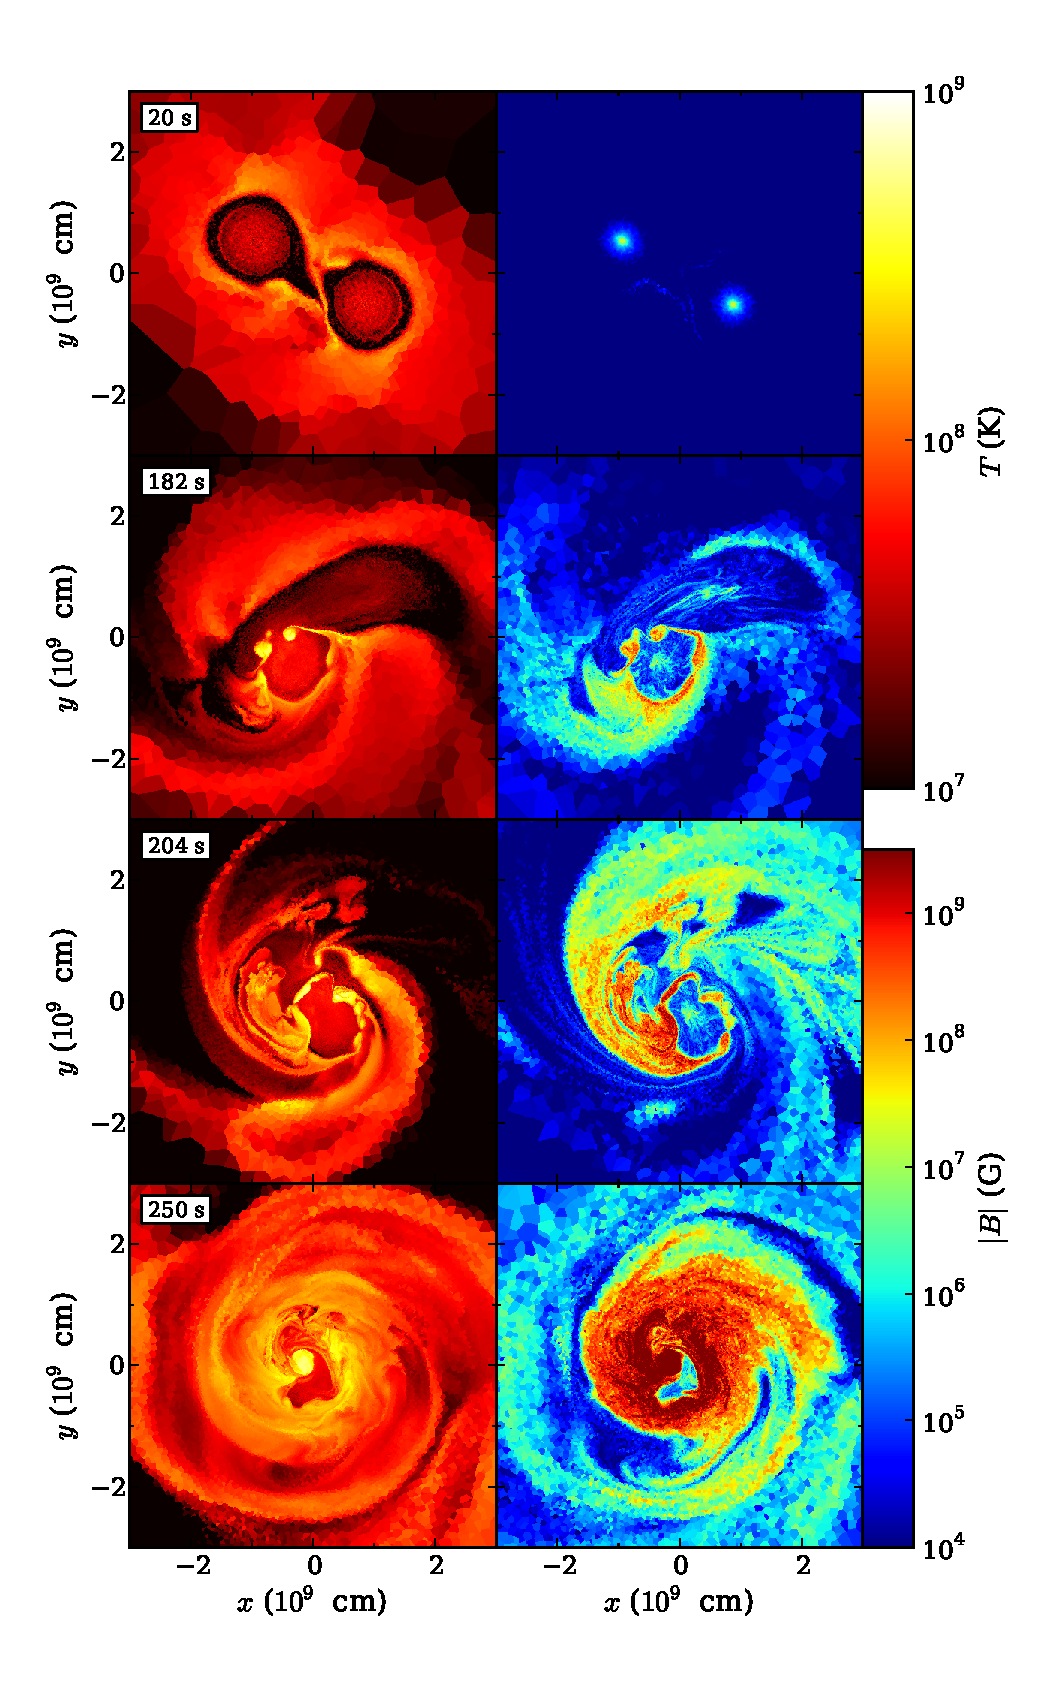
\includegraphics[angle=0,width=0.8\columnwidth]{chapter4_zhu+15/figures/snapshots.pdf}
\caption{Series of temperature $T$ (left column) and magnetic field strength \Bmag\ (right) logarithmic intensity profiles in the equatorial plane of the merger for four snapshots in time (rows; time indicated at the top left of each row).}
\label{fig:c4_snapshots}
\end{figure}

\begin{figure}
\centering
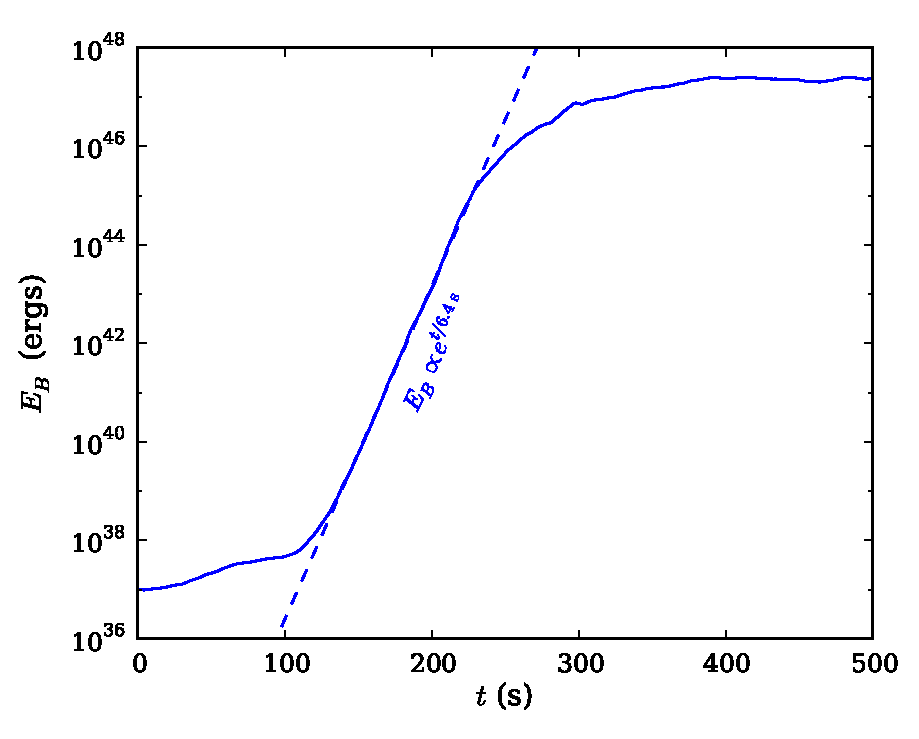
\includegraphics[angle=0,width=0.7\columnwidth]{chapter4_zhu+15/figures/bgrowth.pdf}
\caption{Total magnetic energy \EB\ over time, with a best fit to the rapid exponential growth (dashed $\EB \propto e^{t/6.4\,\mrm{s}}$ line).}
\label{fig:c4_bgrowth}
\end{figure}

We depict the evolution of the binary in Fig. \ref{fig:c4_snapshots}, highlighting temperature $T$ and magnetic field strength \Bmag.  Fig. \ref{fig:c4_bgrowth} shows the growth of total magnetic energy \EB\ over time.

In the first stage of the merger, up to $\sim180$ s, the 0.625 \Msun\ donor WD transfers mass to the 0.65 \Msun\ accretor for about 3.5 orbits before fully disrupting.  Because our initial conditions are approximate -- the WDs are not initially tidally deformed -- mass transfer begins in spurts as the WDs stretch in response to the binary potential, and occurs at a rate that is artificially high \citep{dan+11}.  The early mass transfer shears the atmospheres of both WDs.  As a result, \EB\ grows roughly linearly in the first $\sim100$ s, reaching about quadruple its initial value.  Since the initial mass transfer rate is artificially high, this growth is likely an overestimate, but remains negligible compared to what follows.

%\EB\ could also be a very shallow exponential - the linear fit is marginally better

By $\sim120$ s, mass transfer becomes steady, and a stream of material from the donor wraps around the accretor, forming a shear layer.  Along it, the Kelvin-Helmholtz instability generates a string of hot vortices that exponentially amplify their entrained magnetic fields.  This is illustrated in Fig. \ref{fig:c4_snapshots} (row 2), where the hot vortices along the donor-accretor interface correspond to regions of high field strength.  At $\sim180$ s, tidal forces between the two WDs become strong enough to fully disrupt the donor, which then coalesces with the accretor over $\sim50$ s.  During this time, infalling donor material spirals into the accretor, severely deforming the accretor while carrying the string of magnetized vortices toward the system's center of mass (CM).  Fig. \ref{fig:c4_bgrowth} shows \EB\ growing exponentially by a factor of $\sim10^7$ over $\sim100$ s, with an $e$-folding time $\tau = 6.4$ s, comparable to the typical turnover timescale of the largest eddies $2\pi R_\mrm{eddy}/\Delta v_\mrm{shear} \sim 3\,\mrm{s}$, where $\Delta v_\mrm{shear}$ is the velocity difference across the shear layer.

%2\pi/\Omega_\mrm{eddy} approximated using the three largest eddies in snapshot_092 with 2*pi*r_eddy/v_eddy; r_eddy ~ 1e8 cm, v_eddy ~ 2e8 cm/s.  Similar (slightly smaller) number achieved by looking at the shear layer thickness and delta v.

By $\sim250$ s many of the vortices have merged together into a hot, rapidly rotating underdense void at the CM (Fig. \ref{fig:c4_snapshots}, row 4).  Magnetic growth within the void begins to saturate as its magnetic and kinetic energy approach equipartition.  The rate of field growth slows as well, with \EB\ growing another two orders of magnitude over $\sim150$ s before plateauing at $\sim2\times10^{47}$ ergs at $\sim400$ s.

%Time-averaged E_B between 400 - 500 s to get equilibrium value

\begin{figure}
\centering
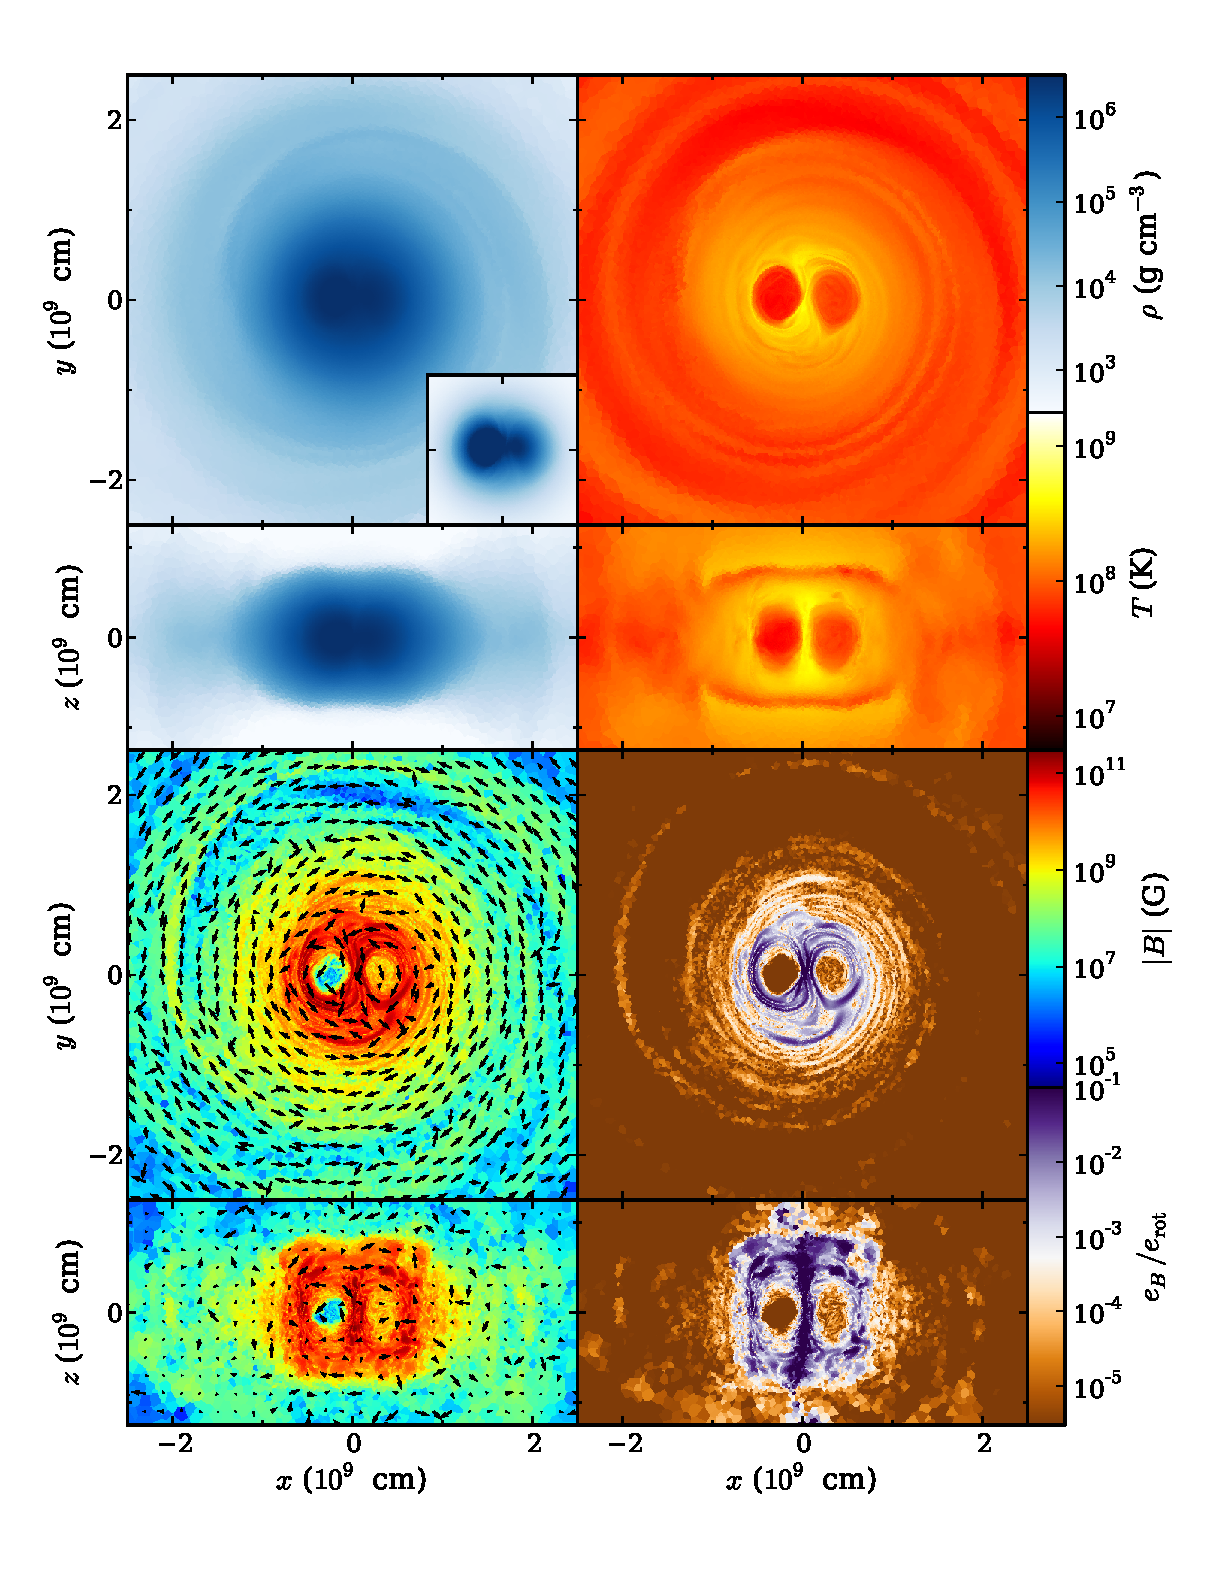
\includegraphics[angle=0,width=0.9\columnwidth]{chapter4_zhu+15/figures/remnant.pdf}
\caption{From leftmost to rightmost column, equatorial plane (top row) and polar (bottom) logarithmic intensity profiles of density $\rho$, temperature $T$, magnetic field strength \Bmag\ and ratio of magnetic to rotational energy density \eberot\ for the simulation at 400 s ($\sim170$ s after coalescence).  The equatorial plane density plot includes a linear profile of the remnant core (with the same $x$ and $y$ scale as the logarithmic profile) to show its shape.  Arrows in the magnetic field strength plots indicate field directions, with their lengths equal to the fraction of the field that lies along the $xy$ plane (top frame) and $xz$ plane (bottom).}
\label{fig:c4_remnant}
\end{figure}

%The core is defined as e_deg/e_tot >= 0.5.  The core essentially consists of all material below r = 7e8 cm, including material at ~3e5 g/cm^3.

In Fig. \ref{fig:c4_remnant} we show the density $\rho$, $T$, \Bmag\ and ratio of magnetic to rotational energy density \eberot\ of the merger remnant at 400 s.  The remnant consists of a dense, degeneracy-supported core containing $\sim60$\% of the remnant's mass, a partly thermally supported hot envelope that surrounds the core, and a rotationally supported disk, a configuration similar to the SPH 0.625-0.65 \Msun\ remnant from Ch. \ref{ch:ch2}.  The \arepo\ remnant core, however, has distinctly non-axisymmetric density and temperature structures, unlike the SPH simulation which achieves axisymmetry $\sim170$ s after coalescence (\citealt{zhu+13}, online figure set Fig. 1.16).  The magnetic fields are too weak during the merger to have an effect on merger dynamics, so these contrasts are due to differences in the \textit{hydrodynamic} schemes between \arepo\ and SPH (Ch. \ref{ch:ch3}).

%From data used in Z13, 2.5% non-axisymmetry is achieved at ~270 s (frame 54000), while coalescence finishes at ~100 s.

%We find running the \arepo\ simulation without any magnetic field still produces a remnant with density and temperature structures similar to those in Fig. \ref{fig:c4_remnant}, and so magnetic fields have a negligible effect on the dynamics of the merger.  Contrasts between the SPH and \arepo\ simulations are due to differences in the \textit{hydrodynamic} schemes between \arepo\ and SPH \Zhuprep.

The remnant magnetic field configuration is complex: while field lines are coherent along ``strands'' of high field strength, neighboring strands often point in opposite directions (see Fig. \ref{fig:c4_remnant}).  In the core, the volume-averaged field strength is $4\times10^{10}$ G, but strands of $>10^{11}$ G field perforate the core.  The field remains $>10^9$ G near the core-disk interface at $\sim 10^9$ cm, before dropping below $10^7$ G at $\gtrsim 3\times10^9$ cm.  The total magnetic field energy is $\sim0.2$\% the total, $\sim0.6$\% the total rotational, and $\sim6$\% the total differential rotation energy of the remnant.\footnote{Differential rotation energy of a cell is estimated with $E_\mrm{drot} = m_\mrm{cell}|\boldsymbol{v}||\nabla\times\boldsymbol{v}|V_\mrm{cell}^{1/3}$.}  This energy is roughly equally partitioned into toroidal and poloidal field components, with the ratio of poloidal to total magnetic energy $\EBphiEB = 0.62$.  Studies of local field amplification within Kelvin-Helmholtz vortices predict magnetic growth saturates when the magnetic and kinetic energy densities are close to equipartition \citep{oberam10, zrakm13}.  In our simulation, this is only the case for the strands of $>10^{11}$ G field, where magnetic energy density is $\sim7$\% ($\sim47$\%) the rotational (differential rotation) energy density (see Fig. \ref{fig:c4_remnant}, column 4).  It is possible that because the strands are distributed throughout the core, they drive the core's overall evolution and inhibit further magnetic amplification in their surroundings.

%In post-merger magnetic amplification scenarios where a dynamo acts upon the inner disk, the field produced remains confined to the inner disk because the diffusion time into the core, $\sim10^9$ yr, exceeds even the remnant thermal cooling time, $\sim10^{7.5}$ yr \citep{garc+12}.  Our fundamentally different configuration results from strong fields being advected into the core during coalescence.  We note, however, that \Bmag\ remains relatively low in the densest parts of the core, and post-merger evolution may shift these regions toward the center, displacing highly magnetized material in the process.

Some of the magnetized accretion stream is ejected during coalescence and integrates into the inner disk ($\sim1 - 3\times10^9$ cm), producing a $10^7 - 10^8$ G field by 400 s.  This field has a negligible hydrodynamic effect on the disk (magnetic energy density to pressure ratio $e_\mrm{B}/P \approx 3\times10^{-5}$ at $2\times10^9$ cm), and, unlike the field in the core, has \textit{not} saturated: \Bmag\ continues to grow exponentially with $\tau \sim 200$ s.\footnote{The remnant disk is generally poorly resolved, even at the highest resolution used in Sec. \ref{ssec:c4_restest}; this may artificially slow the disk field growth rate.}
